
\myPara{High-quality}
% \dq{@Jodai}
We also perform a fine-tuning process to enhance the spatial quality of the generated videos. As illustrated in Figure \ref{fig:high_quality}, \nameofmethod{} is capable of producing videos with ultra-detailed content.
\begin{figure}[!htbp]
    \centering
    \begin{subfigure}{\textwidth}
        \centering
        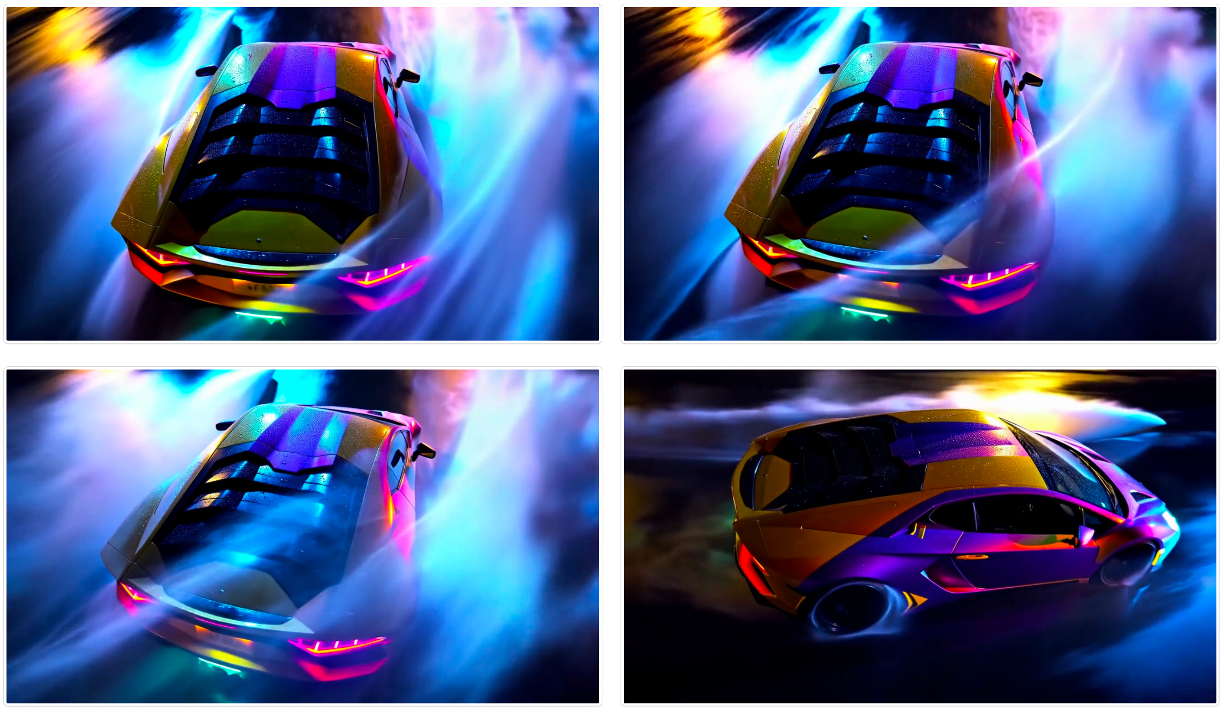
\includegraphics[width=\textwidth]{figures/high-quality-1.png}
        \caption{Prompt: the ultra-wide-angle lens follows closely from the hood, with raindrops continuously splattering against the lens. Ahead, a sports car speeds around a corner, its tires violently skidding against the wet road, creating a mist of water. Neon lights refract in the rain, leaving colorful streaks on the car's surface. The camera swiftly shifts to the side of the car, capturing the wheels spinning at high speed, before finally moving to the rear.}
    \end{subfigure}
    \hfill
    \begin{subfigure}{\textwidth}
        \centering
        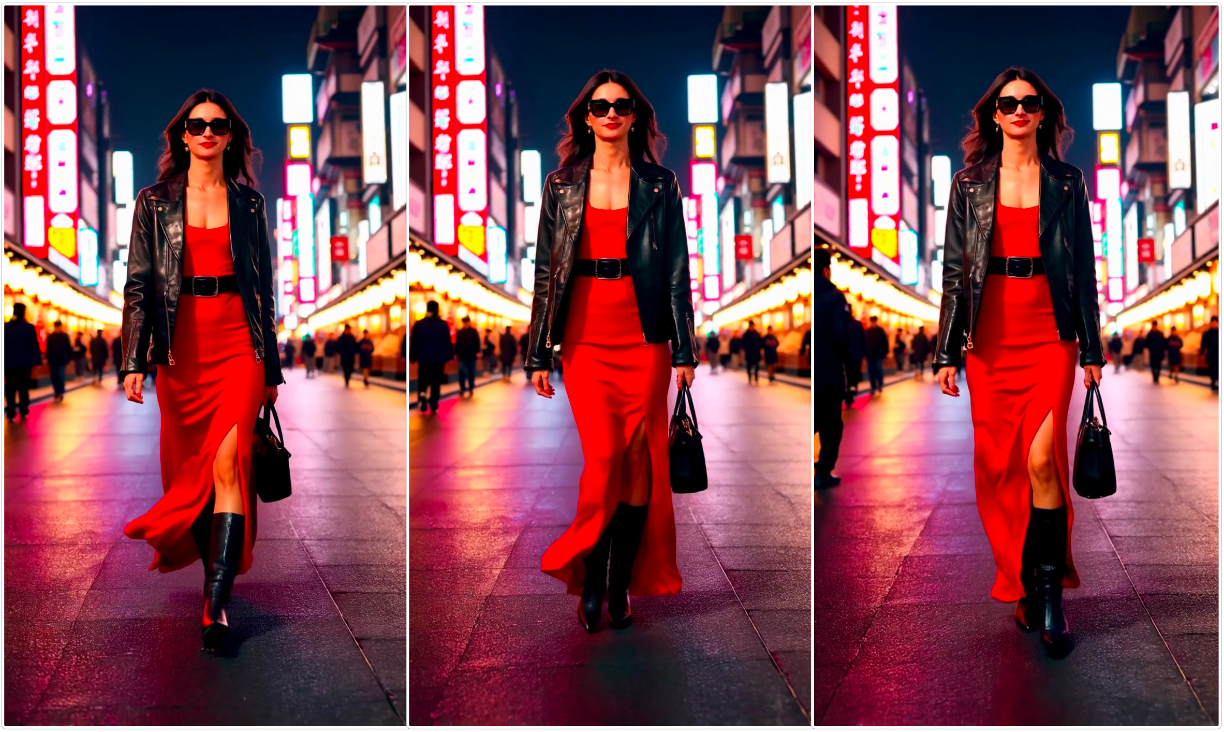
\includegraphics[width=\textwidth]{figures/high-quality-2.png}
        \caption{Prompt: a stylish woman walks down a Tokyo street filled with warm glowing neon and animated city signage. She wears a black leather jacket, a long red dress, and black boots, and carries a black purse. She wears sunglasses and red lipstick. She walks confidently and casually. The street is damp and reflective, creating a mirror effect of the colorful lights. Many pedestrians walk about.}
    \end{subfigure}
    \caption{High-quality videos generated by HunyuanVideo.}
    \label{fig:high_quality}
\end{figure}

\myPara{High-motion Dynamics}
% \dq{@Weijie, Junkun}
In this part, we demonstrate \nameofmethod{}'s capabilities in producing high-dynamic videos based on given prompts. As shown in Figure \ref{fig:high_motion}, our model excels in generating videos that encompass a wide range of scenes and various types of motion.

\begin{figure}[!htbp]
    \centering
    \begin{subfigure}{\textwidth}
        \centering
        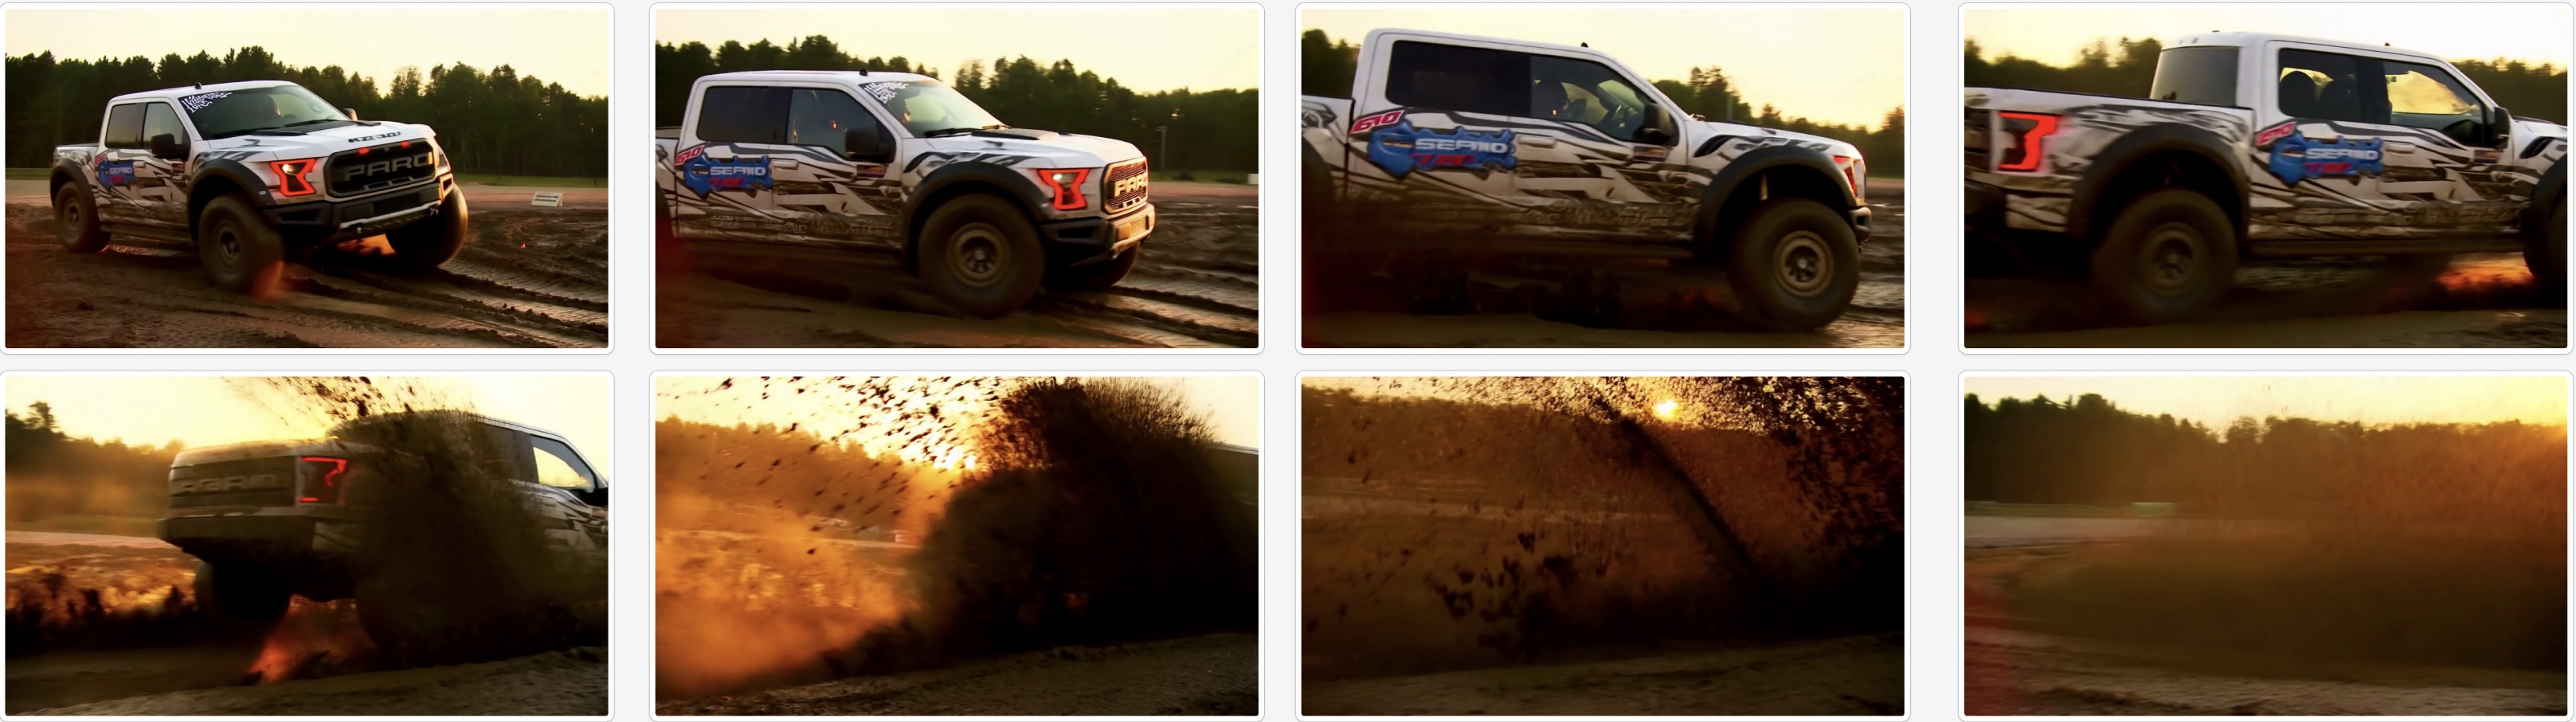
\includegraphics[width=\textwidth]{figures/high_motion_3.jpg}
        \captionsetup{font=small}
        \caption{Prompt: At sunset, a modified Ford F-150 Raptor roared past on the off-road track. The raised suspension allowed the huge explosion-proof tires to flip freely on the mud, and the mud splashed on the roll cage.}
        \label{fig:hm_1}
    \end{subfigure}
    \hfill
    \begin{subfigure}{\textwidth}
        \centering
        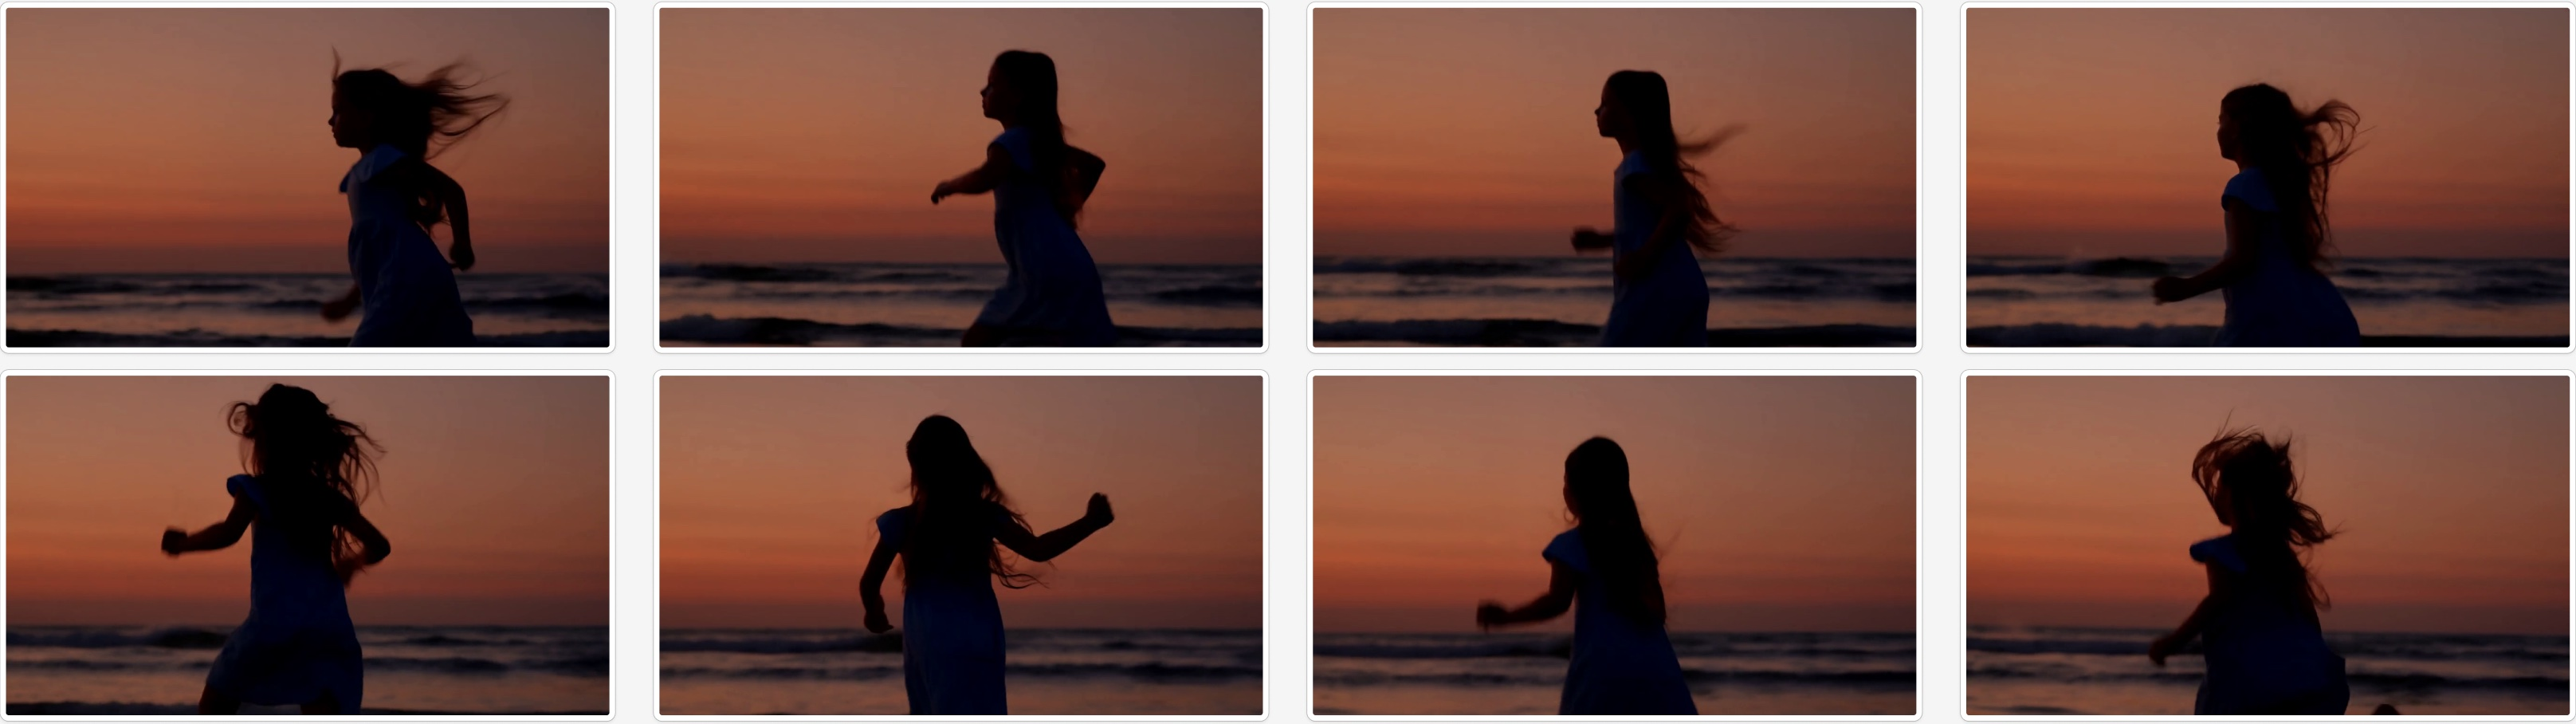
\includegraphics[width=\textwidth]{figures/high_motion_5.jpg}
        \captionsetup{font=small}
        \caption{Prompt: The panning camera moves forward slowly, with a depth of field in the middle focus, and warm sunset light covers the screen. The girl in the picture runs with her skirt fluttering, turns and jumps.}
        \label{fig:hm_2}
    \end{subfigure}
    \hfill
    \begin{subfigure}{\textwidth}
        \centering
        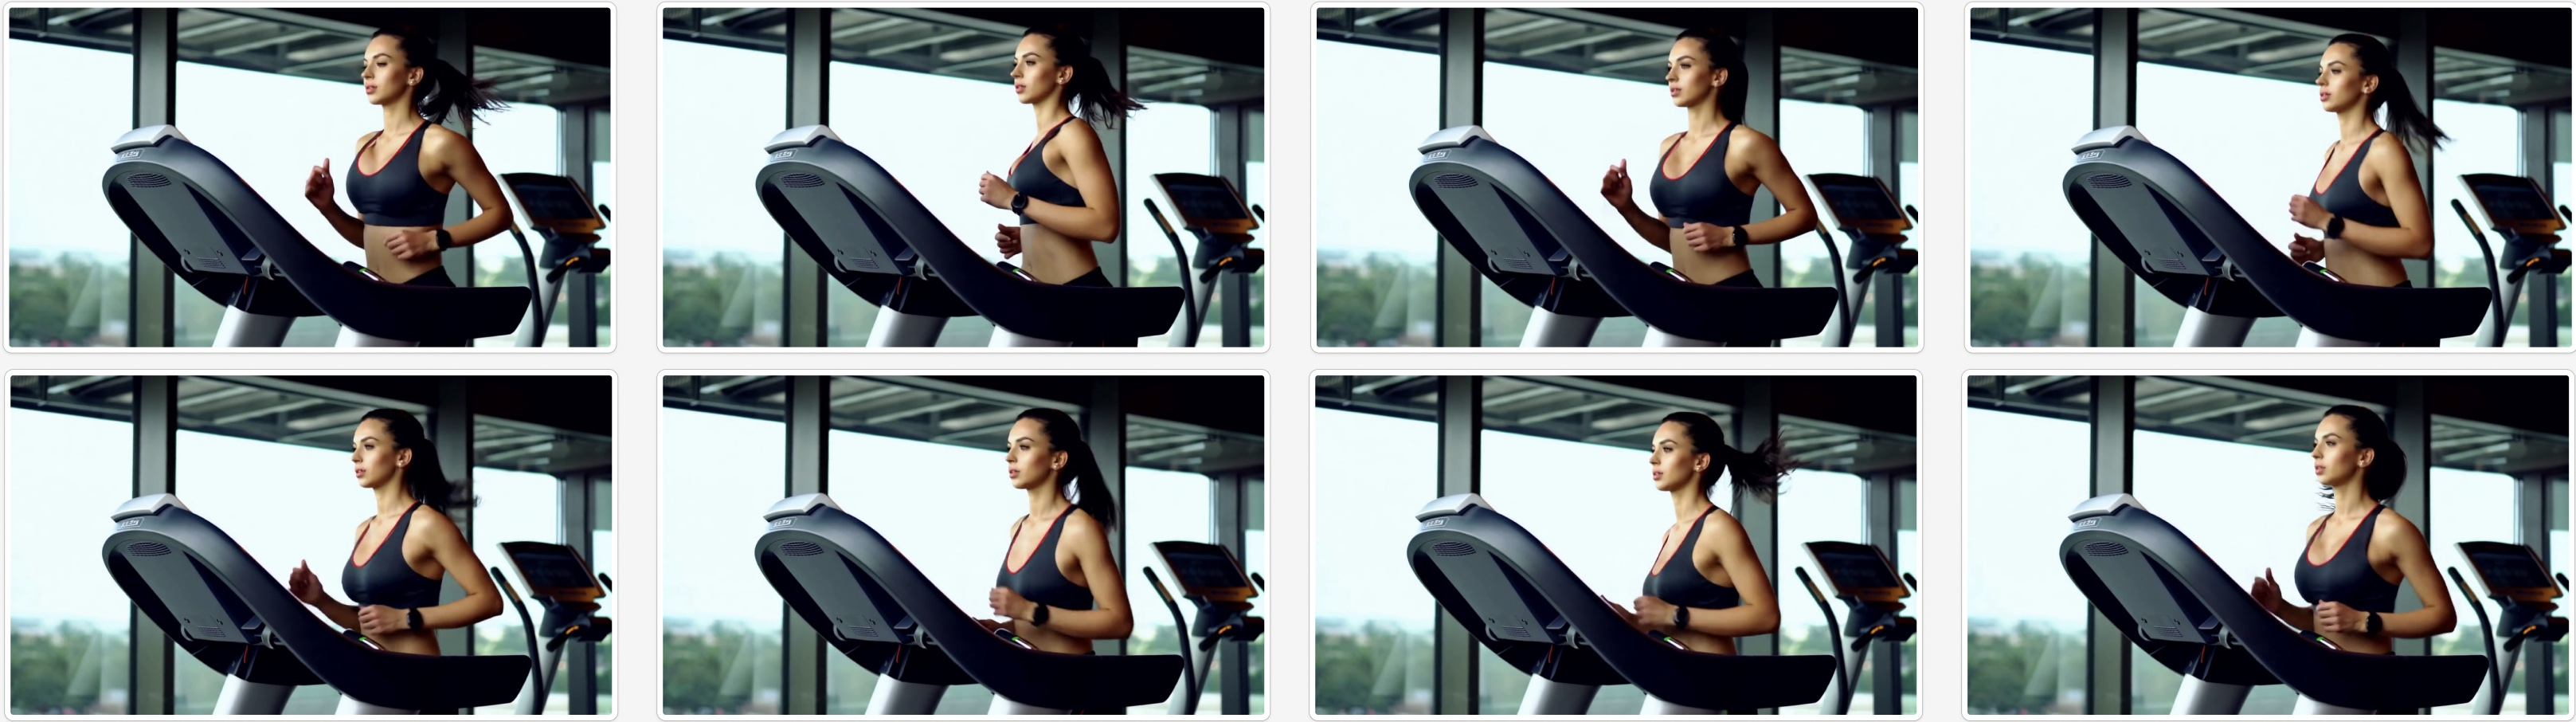
\includegraphics[width=\textwidth]{figures/high_motion_2.jpg}
        \captionsetup{font=small}
        \caption{Prompt: In the gym, a woman in workout clothes runs on a treadmill. Side angle. Realistic, Indoor lighting, Professional.}
        \label{fig:hm_3}
    \end{subfigure}
    \hfill
    \begin{subfigure}{\textwidth}
        \centering
        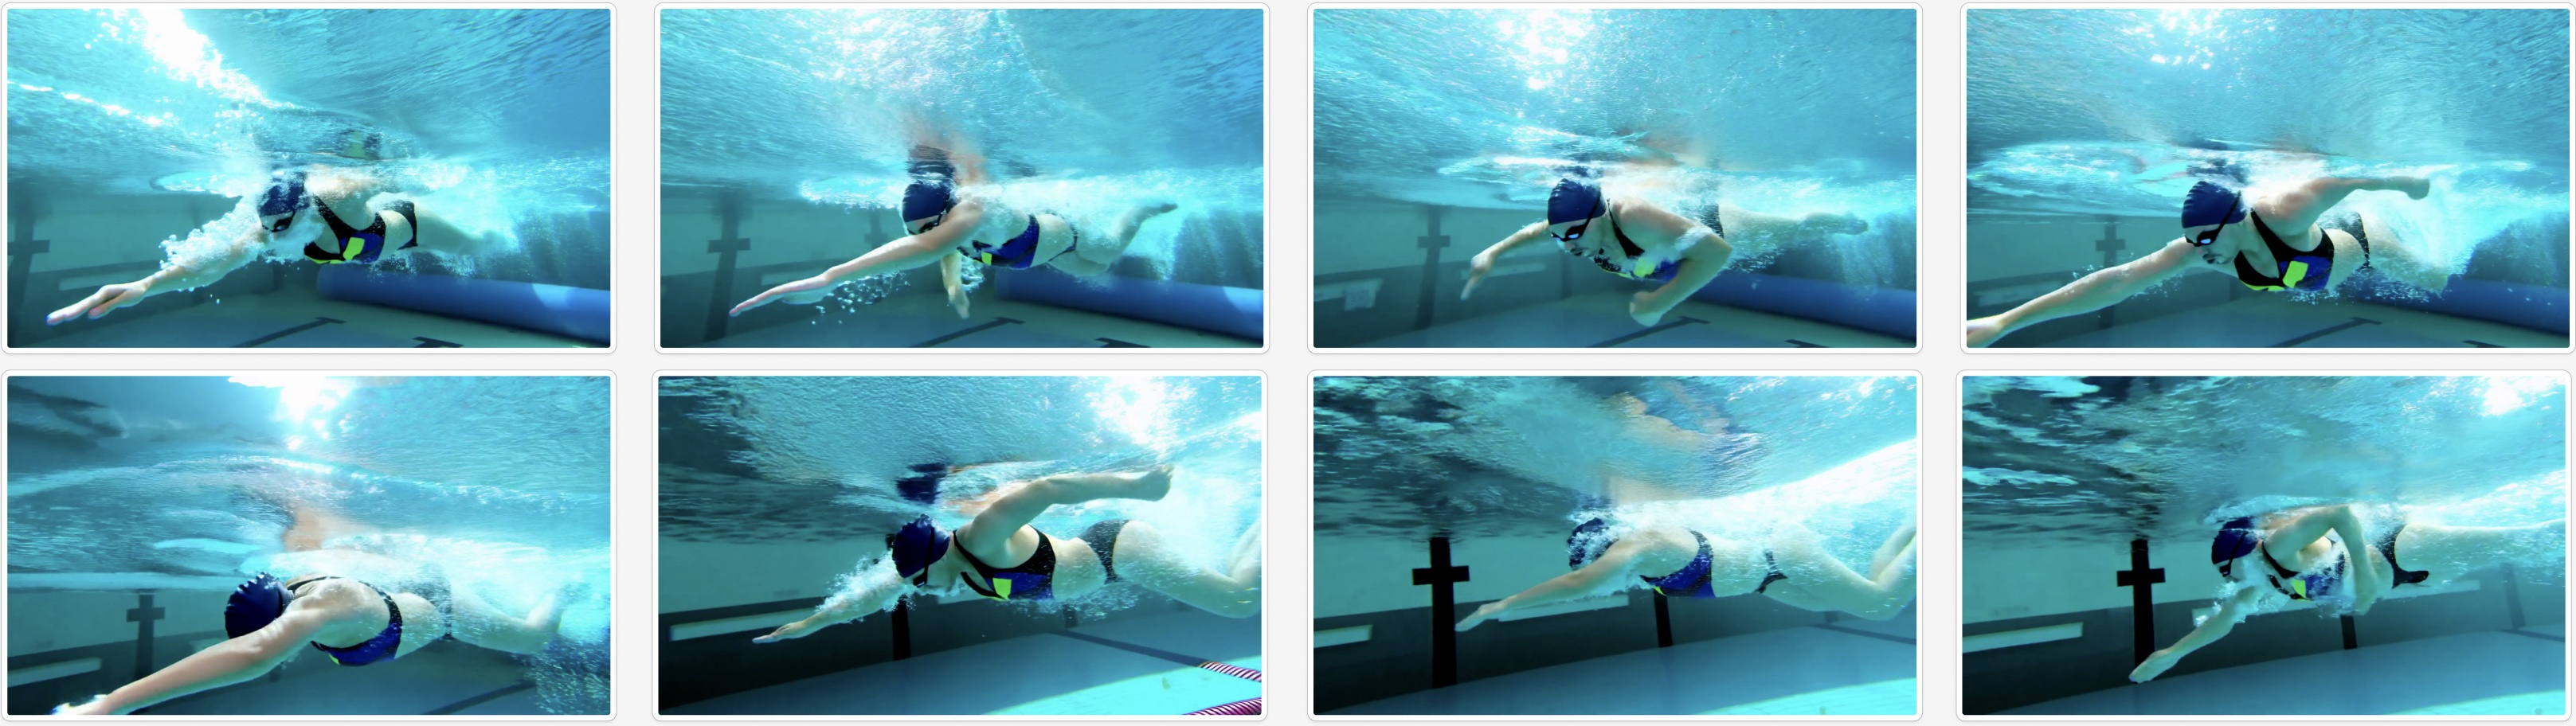
\includegraphics[width=\textwidth]{figures/high_motion_7.jpg}
        \captionsetup{font=small}
        \caption{Prompt: Swimmer swimming underwater, in slow motion. Realistic, Underwater lighting, Peaceful.}
        \label{fig:hm_4}
    \end{subfigure}
    \hfill
    \begin{subfigure}{\textwidth}
        \centering
        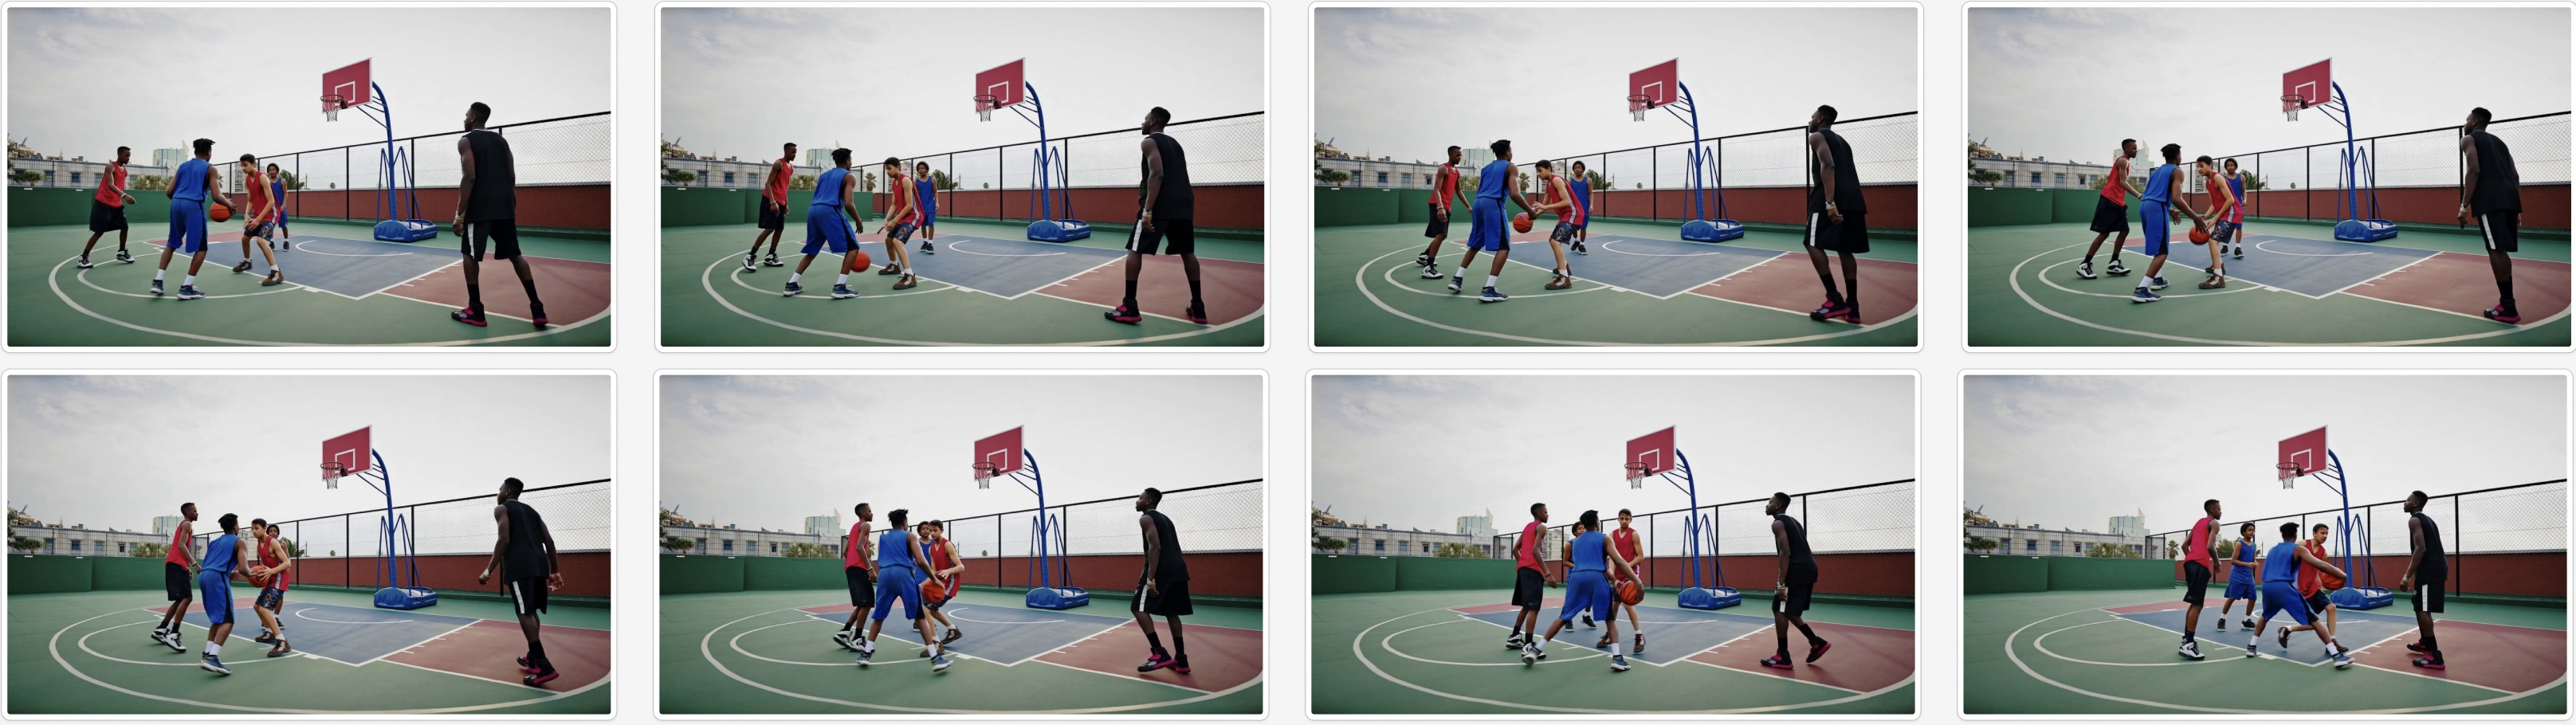
\includegraphics[width=\textwidth]{figures/high_motion_8.jpg}
        \captionsetup{font=small}
        \caption{Prompt: On the rooftop, there is an open-air basketball court, and five male students are playing basketball. Realistic, Natural lighting, Casual.}
        \label{fig:hm_5}
    \end{subfigure}
    \caption{High-motion dynamics videos generated by \nameofmethod{}.}
    \label{fig:high_motion}
\end{figure}


\myPara{Concept Generalization}
% \dq{@Daquan, Zhiyu}
One of the most desirable features of a generative model is its ability to generalize concepts. As illustrated in Figure \ref{fig:concept}, the text prompt describes a scene: "In a distant galaxy, an astronaut floats on a shimmering, pink, gemstone-like lake that reflects the vibrant colors of the surrounding sky, creating a stunning scene. The astronaut gently drifts on the lake's surface, while the soft sounds of water whisper the planet's secrets. He reaches out, his fingertips gliding over the cool, smooth water." Notably, this specific scenario has not been encountered in the training dataset. Furthermore, it is evident that the depicted scene combines several concepts that are also absent from the training data.
\begin{figure}[!htbp]
    \centering
    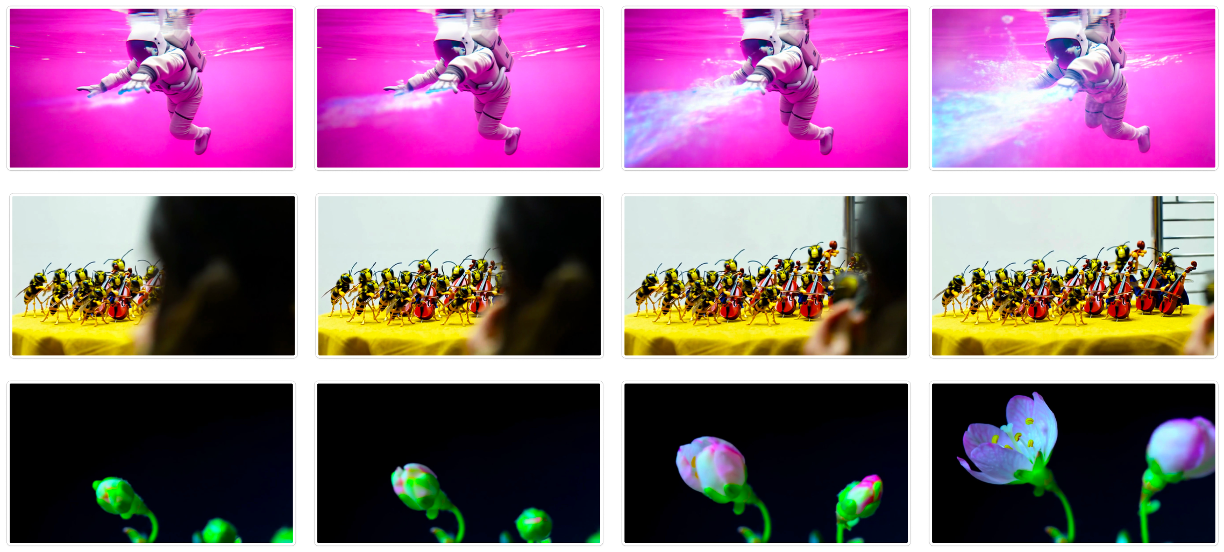
\includegraphics[width=\linewidth]{figures/concept.png}
    \caption{\small {\nameofmethod{}'s performance on concept generalization. The results of the three rows correspond to the text prompts (1) `In a distant galaxy, an astronaut floats on a shimmering, pink, gemstone-like lake that reflects the vibrant colors of the surrounding sky, creating a stunning scene. The astronaut gently drifts on the lake's surface, the soft sounds of water whispering the planet's secrets. He reaches out, his fingertips gliding over the cool, smooth water. ', (2) `A macro lens captures a tiny orchestra of insects playing instruments.' and (3) `The night-blooming cactus flowers in the evening, with a brief, rapid closure. Time-lapse shot, extreme close-up. Realistic, Night lighting, Mysterious.' respectively.} }
    \label{fig:concept}
\end{figure}

\myPara{Action Reasoning and Planning}
% \dq{@Li Xin}
Leveraging the capabilities of large language models, \nameofmethod{} can generate sequential movements based on a provided text prompt. As demonstrated in Figure \ref{fig:sequential-move}, \nameofmethod{} effectively captures all actions in a photorealistic style.
\begin{figure}[ht]
    \centering
    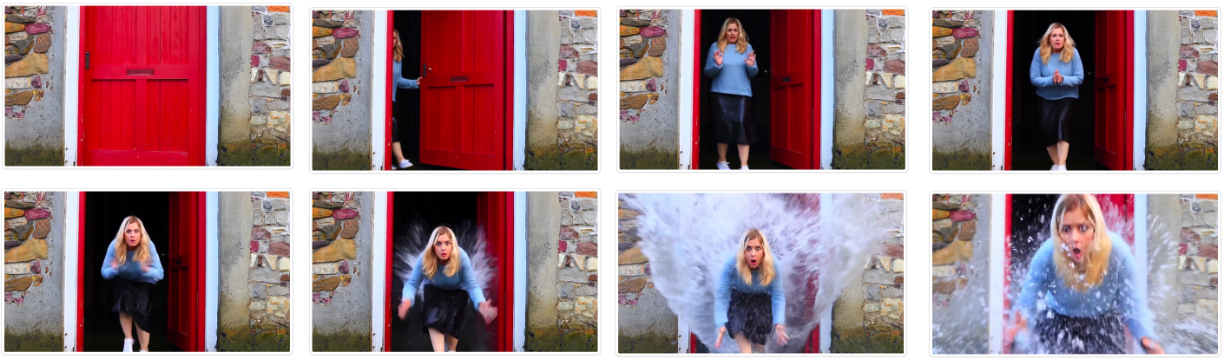
\includegraphics[width=\linewidth]{figures/sequential_motion.png}
    \caption{{Prompt: The woman walks over and opens the red wooden door. As the door swings open, seawater bursts forth, in a realistic style.}}
    \label{fig:sequential-move}
\end{figure}

\myPara{Character Understanding and Writing}
\nameofmethod{} is capable of generating both scene text and gradually appearing handwritten text as shown in Fig.~\ref{fig:ocr}. 



% \dq{@Wuyue}
\begin{figure}[!htbp]
    \centering    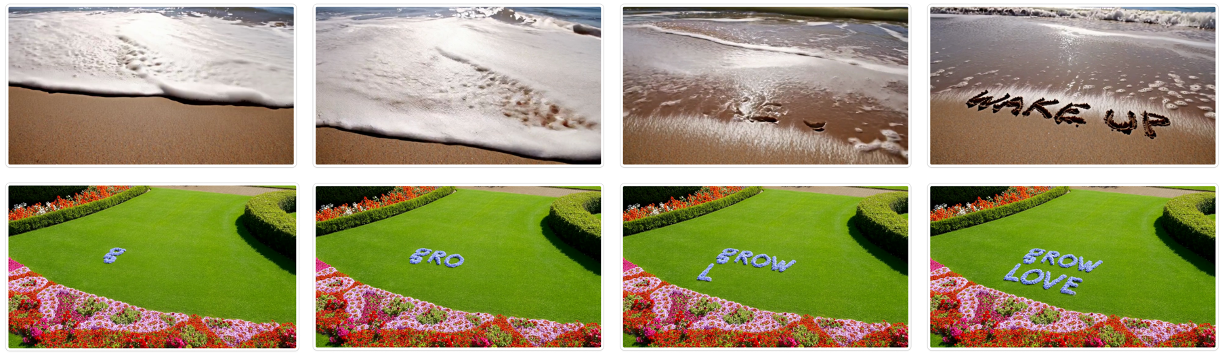
\includegraphics[width=\linewidth]{figures/ocr.png}
    \caption{High text-video alignment videos generated by HunyuanVideo. Top row: Prompt: A close-up of a wave crashing against the beach, the sea foam spells out ``WAKE UP'' on the sand. Bottom row: Prompt: In a garden filled with blooming flowers, ``GROW LOVE'' has been spelled out with colorful petals.}
    \label{fig:ocr}
\end{figure}



